\section{Méthodes possibles pour la virtualisation légère}
\label{section:emulation}

Il existe actuellement deux méthodes permettant de faire de la virtualisation
légère. La première est une émulation par limitation ou dégradation également
appelée virtualisation standard et la seconde est une émulation par
interception.

\subsection{Virtualisation standard}
%% \begin{itemize}
%% \item principe: limiter l'accès aux ressources par exemple (cgroup, netstat, cpuburner), temps d'un SEB (bench avec netlink, limiter (cap))
%% \item avantage plus simple
%% \item désavantages: host>>target, modèle à vérifier, contrôle expérimental fin
%% \end{itemize}
Avec cette première méthode on place la couche d'émulation au-dessus de la
plate-forme réelle (comme un hyperviseur pour une VM). De fait, la puissance de
l'émulateur dépend de la puissance de la machine hôte et ne peux pas dépasser
les capacités de cette dernière. En effet, des machines plus puissantes que
l'hôte répondrait plus rapidement que ce dernier à une demande d'une
application. Or le délai de réponse géré par l'émulateur ne peut-être inférieur
à celui de l'hôte sinon l'hôte n'aurait pas le temps de faire les calculs
demandés et de répondre à l'émulateur qui répondrait à l'application. De plus,
en choisissant de placer l'émulation comme une sur-couche cela permet de limiter
l'accès aux ressources pour les applications. En effet les applications ne
pourront pas passer la couche d'émulation pour accéder aux ressources localisées
sur la machine hôte. Les requêtes des applications distribuées seront arrêtées
par l'émulateur. C'est lui qui s'occupera de récupérer les ressources demandées
par les applications. Il existe différent outils permettant de faire de mettre
en place cette virtualisation, on trouve notamment \textbf{cgroup},
\textbf{netstat} et \textbf{cpuburner}.  Cette solution a l'avantage d'être
simple à mettre en \oe uvre puisque l'on se basse sur la machine hôte. Néanmoins
elle est assez contraignante du fait qu'on ne puisse pas émuler des
architectures plus performantes que l'hôte. De plus {\color{red} à écrire deux
  derniers points négatifs à éclaircir}.

\subsection{Émulation par interception}
%% principe: interception des actions et médiation (pas juste interception et rejeu). Intercepter des symboles pour en changer l'effet

Dans le cas de l'émulation par interception, pour faire croire à l'application
qu'elle s'exécute sur une machine autre que l'hôte on va utiliser deux outils;
un simulateur pour virtualiser l'environnement d'exécution et un émulateur qui
va attraper toutes les communications de l'application avec l'hôte et qui les
transmettra ensuite au simulateur. Les calculs de l'application seront effectués
sur la machine hôte mais c'est le simulateur qui calculera le temps de réponse à
l'application. Pour cela il fera un rapport entre le temps d'exécution du calcul
sur la machine hôte (fourni par l'émulateur qui le mesure lors de l'exécution du
calcul), la puissance de l'hôte et celle des machines de l'environnement que
l'on simule. Le temps de l'application sera donc celui du simulateur et non le
temps réel. En effet, l'application quand elle fait un calcul pense être sur une
autre machine avec des performances différentes, elle est donc capable de savoir
combien de temps prends une certain calcul sur son architecture. Hors sur l'hôte
ce calcul ne prendra pas le même temps et l'application se retrouvera avec un
temps prévu et un temps qui ne correspondent pas ce qui est problématique.  Avec
cette solution on ne se contente pas de faire de l'interception d'action et du
rejeu par l'émulateur comme c'est le cas avec l'émulation par limitation. On va
intercepter les actions des applications et faire de la médiation, autrement dit
on va modifier les actions avant de les laisser s'exécuter sous le contrôle de
l'émulateur.

 Une application distribuée peut vouloir communiquer avec l'hôte soit pour
 effectuer de simples calculs (SEB), soit pour effectuer des requêtes de
 connexion ou de communication avec d'autres applications sur le réseau. Quand
 l'émulateur intercepte une communication venant d'un des processus d'une
 application, il modifie les caractéristiques de cette dernière pour qu'elle
 puisse s'exécuter sur la machine hôte. Quand la machine hôte renvoie une
 réponse à l'application, elle est également interceptée par l'émulateur pour
 que l'application ne voit pas le changement d'architecture. En même temps, il
 envoie au simulateur des données concernant le temps d'exécution de l'action
 sur la machine hôte pour qu'il puisse calculer le temps d'exécution sur la
 machine simulée. Les délais calculés par le simulateur sont soit des temps de
 calculs soit des temps de connexion. \textit{Quand le simulateur a terminé le
   calcul du temps de réponse nécessaire il l'envoie à l'émulateur qui l'envoie
   à l'application en plus du résultat du calcul demandé afin de mettre à jour
   l'horloge de l'application.} Ainsi les calculs sont réellement exécutés sur
 la machine, les communications réellement émises sur le réseau géré par le
 simulateur et c'est le temps de réponse fourni par le simulateur qui va
 influencer l'horloge de l'application permettant ainsi d'imiter un
 environnement distribué. Finalement les applications ne communiquent plus
 directement entre elles puisque toute communication est interceptée par
 l'émulateur, puis gérée par le simulateur qui s'occupe du réseau.

{\color{red} Mettre deux schémas de action interceptes, test modifie, renvoie,
  attrape réponse, simulateur, retour application, un quand simple calcul
  l'autre quand connexion}

Pour intercepter ces actions, il faut d'abord choisir à quel niveau se place
l'interception: code source ou binaire. Mais il faut également choisir sur quel
type de symbole utilisée par l'application pour exécuter ses actions se fera la
médiation qui suit l'interception et avec quel outil. En effet une application
peut communiquer avec le noyau via différentes abstractions. Elle peut soit
utiliser les fonctions d'interaction directe avec le noyau que sont les appels
systèmes, soit utiliser les différentes abstractions fournies par le système
d'exploitation: bibliothèques (fonctions systèmes de la libc par exemple) ou les
fonctions POSIX dans le cas d'un système UNIX.

\begin{figure}[H]
 \centering
 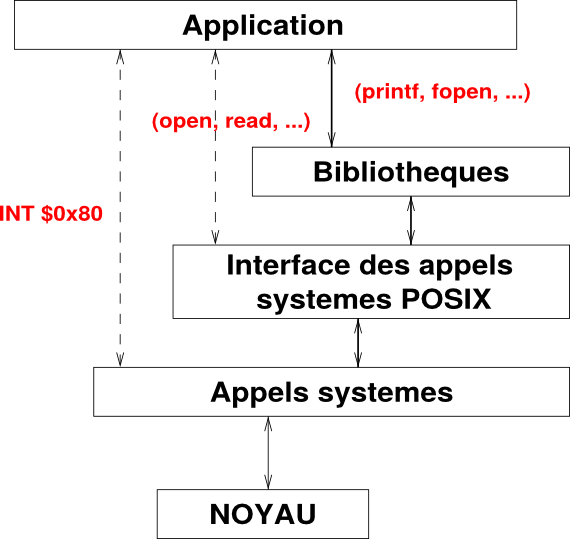
\includegraphics[scale=0.5]{Pictures/Communication_application_noyau_v1.png}
 \caption{Communications possibles entre le noyau et une application}
 \label{AS_Communication}
\end{figure}

Nous allons donc voir comment on peut faire de l'interception sur un fichier
source puis sur un binaire, puis nous verrons comment faire de la médiation sur
différents symboles: appels de fonctions et appels systèmes.
%% {\color{red} L'interception des actions d'une application peut se faire à deux niveaux: sur le fichier source et sur le binaire. La médiation qui suit l'interception des actions peut également se faire sur différent type de symboles: les appels de focntions et les appels systèmes.  \textit{mettre partie ce qu'on intercepte pourquoi et le schéma}}

\subsubsection{Action sur le fichier source}
%% reimplem SMPI (trop spé) ,source to source/ pass LLVM( gcc+libc=consanguin) 
%% , Coccinelle

\subsubsection{Action sur le binaire}
%%Valgrind (perf pourrie)
Pour agir sur le binaire d'une application, c'est l'outil de programmation libre Valgrind\cite{INTERCEPTION:Valgrind, INTERCEPTION:Valgrind_web} que nous allons étudier. À l'origine c'est un outil de programmation pour le débuguage mémoire, puis il a évolué pour devenir l'instrument de base à la création d'outils d'analyse dynamique de code, tels que la mise en évidence de fuites mémoires et le profilage de code\footnote{Méthode visant à analyser le code d'une application pour connaître la liste des focntions appelées et le temps passé dans chacune d'elles}. Valgrind fonctionne à la manière d'une machine virtuelle faisant de la compilation à volée\footnote{Technique basée sur la compilation de byte-code et la compilation dynamique. Elle vise à améliorer la performance de systèmes bytecode-compilés par la traduction de bytecode en code machine natif au moment de l'exécution}. Ainsi, ce n'est pas le code initial du programme qu'il envoie au processeur de la machine hôte. Il traduit d'abord le code dans une forme simple appelée ``Représentation Intermédiaire'' en compilation. Ensuite, un des outils d'analyse dynamique de Valgrind peut être utilisé pour faire des transformations sur cette ``Représentation Intermédiaire''. Pour finir, Valgrind traduit la ``Représentation Intermédiaire'' en langage machine et c'est ce code que le processeur de la machine hôte va exécuter. De plus, grâce à la compilation dynamique, Valgrind peut recompiler certaines parties du code d'un programme durant son exécution et donc ajouter de nouvelles fonctions au code de l'application en cours d'exécution.

Dans notre cas, on pourrait l'utiliser pour mesurer le temps passé à faire un calcul, qui serait ensuite envoyé au simulateur pour calculer le temps de réponse dans l'environnement simulé nécessaire à l'émulateur. On pourrait également l'utiliser pour réécrire à la volée le code des fonctions que l'émulateur doit modifier pour maintenir la virtualisation. Pour faire cela, il faut créer un ``wrapper'' pour chaque fonction qui nous intéresse. Un wrapper dans Valgrind est une fonction de type identique à celle que l'on souhaite intercepter, mais ayant un nom différent (généré par les MACRO de Valgrind) pour la différencier de l'originale. Pour générer le nom du wrapper avec les macro de Valgrind on doit préciser la bibliothèque qui contient la fonction originale et utiliser un encodage spécifique à Valgrind. Cette opération est lourde et complexe. De plus, elle nécessite de connaître le nom de la bibliothèque qui contient la fonction qui nous intéresse. Cette solution est donc assez contraignante et ses performances sont assez médiocres d'après l'étude faite par M. Guthmuller lors de son stage \cite{INTERCEPTION:MARION}: facteur de 7.5 pour le temps d'exécution d'une application avec cet outil. Cette perte de performance est due à la compilation faite en deux phases ainsi qu'au temps nécessaire aux outils de Valgrind pour modifier ou rajouter du code à l'existant. Cela pourrait être acceptable, si Valgrind faisait de la traduction dynamique lors de la seconde phase de sa compilation, nous permettant ainsi d'avoir du code exécutable sur un autre type de processeur que celui de l'hôte, mais ce n'est pas le cas. 

\subsubsection{Médiation des Appels Système}
%% pourquoi: read/write, comm reseau 

En regardant la Fig.\ref{AS_Communication}, et les différents niveaux
d'abstractions, le moyen plus simple pour attraper les actions de l'application
en gérant un minimum de choses serait d'intercepter directement les appels
systèmes.  Ces derniers sont constitués de deux parties; la première, l'entrée,
initialise l'appel via les registres de l'application qui contiennent les
arguments de l'appel puis donne la main au noyau. La seconde, la sortie, inscrit
la valeur de retour de l'appel système dans le registre de retour de
l'application, les registres d'arguments contenant toujours les valeurs reçues à
l'entrée de l'appel système, et rend la main à l'application. Nous devons donc
intercepter les deux parties de l'appel système pour maintenir notre
environnement simulé et donc stopper l'application à chaque fois pour récupérer
ou modifier les informations nécessaires avant de lui rendre la main pour entrer
ou sortir de l'appel système.

 Nous allons donc voir comment il est possible de faire cela, puisque de
 nombreux outils existent.
 
 \paragraph{L'appel système ptrace}\cite{INTERCEPTION:AS, INTERCEPTION:MARION}
 permet de tracer tous les événement désirés d'un processus, mais aussi d'écrire
 et de lire directement dans l'espace d'adressage de ce dernier, à n'importe
 quel moment ou lorsque un événement particulier se produit. De cette façon on
 peut contrôler l'exécution d'un processus. C'est un appel système unique dont
 chaque action à effectuer est passée sous forme de requêtes en paramètre de
 l'appel système.

Pour pouvoir contrôler un processus via ptrace on va créer deux processus
parents via un \textit{fork()}; un processus appelé ``processus espionné'' qui
exécutera l'application et qu'on souhaite contrôler, et un autre qui contrôlera
le processus espionné, appelé ``processus espion''. Le processus espionné
indiquera au processus espion qu'il souhaite être contrôlé via un appel système
ptrace et une requête PTRACE\_TRACEME puis il exécutera l'application via un
\textit{exec()}. À la réception de cet appel le processus espion notifiera son
attachement au processus espionné via un autre appel à ptrace et une requête
PTRACE\_ATTACH. Il indiquera également sur quelles actions du processus espionné
il veut être notifié (chaque instruction, signal, sémaphore...), définissant
ainsi les actions bloquantes pour le processus espionné. Dans notre cas, ce
seront les appels systèmes que l'on considérera comme points d'arrêts pour le
processus espionné (requête PTRACE\_SYSCALL). Ainsi, le processus espion sera
donc appelé deux fois: à l'entrée et à la sortie de l'appel système. De fait,
quand un des processus de l'application voudra faire un appel système quelconque
il sera bloqué avant de l'exécuter, un appel système ptrace sera lancé et
notifiera le processus espion lié au processus espionné. L'espion fera les
modifications nécessaires dans les registres du processus espionné pour
conserver la virtualisation de l'environnement grâce aux requêtes PEEK\_DATA et
POKE\_DATA passées en argument de l'appel système {\color{red}ou en modifiant
  directement le contenu du /proc/id/mem}. Puis, il rendra la main au processus
espionné bloqué pour que l'appel système puisse avoir lieu. Au retour de l'appel
système le processus espionné sera de nouveau stoppé, un ptrace sera envoyé au
processus espion qui remodifiera les informations nécessaires. Puis il rendra la
main au processus espionné bloqué qui sortira de son appel système avec un
résultat exécuté sur la machine hôte et un temps d'exécution et une horloge
fournie par le simulateur. Quand un processus espion a fini un suivi, il peut
envoyer deux types de requêtes au processus espionné: PTRACE\_KILL qui termine
le processus espionné ou PTRACE\_DETACH qui le laisse continuer son exécution.

{\color{red} Mettre un schéma attachement attente père attrape signal
  modification main fils as retour père et vérification noyau...}

Néanmoins, pour contrôler un processus ptrace fait de nombreux changements de
contexte pour pouvoir intercepter et gérer les événements. De plus il supporte
mal les processus utilisant du multithreading, et ne fait pas parti de la norme
POSIX donc son exécution peut varier d'une machine à une autre.

\paragraph{Uprobes}\cite{INTERCEPTION:AS, INTERCEPTION:MARION}
%% Non module noyau
pour \textit{user-space probes}, quant à lui est une API noyau, également appelé
module d'instrumentation, permettant d'insérer dynamiquement des points d'arrêts
à n'importe quel endroit dans le code d'une application, dans notre cas les
appels systèmes. Pour chaque point d'arrêt l’utilisateur fournit un handler
particulier à exécuter avant ou après l’instruction marquée. Uprobes étant un
outil s'exécutant dans le noyau les handlers doivent être des modules. Pour
chaque point d'arrêt géré par Uprobes, on a donc un module noyau qui contient le
handler à exécuter, ainsi que le processus et l'adresse virtuelle du point
d'arrêt. Lorsqu'un point d'arrêt est atteint Uprobes prend la main et exécute le
bon handler. Pour savoir qu'un point d'arrêt a été touché Uprobes utilise Utrace
équivalent de ptrace en mode noyau qui permet d'éviter les nombreux changements
de contexte et qui est capable de gérer le multithreading. Utrace peut également
être utilisé dans le module gérant un point d'arrêt pour récupérer des
informations sur l'application et les données qu'elle utilise.

Les deux avantages de l'API noyau est qu'elle est rapide et qu'elle a accès à
toutes les ressources sans aucune restriction. Mais ce dernier point représente
aussi son plus gros défaut de par sa dangerosité. De plus, dans notre cas il ne
semble pas judicieux de faire de la programmation noyau via des modules dont il
faudra également gérer le bon chargement.

\paragraph{Seccomp/BPF:}
%% Read only
Seccomp \cite{INTERCEPTION:seccomp_bpf} est un appel système qui permet d'isoler
un processus en lui donnant le droit d'appeler et d'exécuter qu'un certain
nombre d'appels systèmes: \textit{read}, \textit{write}, \textit{exit} et
\textit{sigreturn}. Si le processus fait un autre appel système, tout le
processus sera arrêté avec un signal \textit{SIGKILL}. Comme cela est assez
contraignant, le nombre d'applications que l'on peut utiliser avec seccomp est
donc très limité. Pour plus de flexibilité, on peut utiliser une extension de
cet appel système appelée seccomp/BPF, pour \textit{seccomp Berkeley Packet
  Filter}. Cette dernière permet de définir dans un programme BPF \footnote{Le
  programme fonctionne comme pour les sockets, mais dans notre cas les données
  sur lesquelles on applique les filtres ne sont plus les paquets réseaux mais
  les appels systèmes} \cite{INTERCEPTION:bpf} les appels systèmes autorisés à
s'exécuter. Les filtres sont créés sous forme d'arborescence, quand on rajoute
un filtre on rajoute un noeud. Pour chaque filtre ajouté il faut resynchronyser
les processus utilisant cette arborescence pour filtrer leurs appels
systèmes. Pour pouvoir s'exécuter un appel système doit pouvoir passer à travers
toutes les règles. Dans le cas où les appels systèmes \textit{fork()} ou
\textit{clone()} peuvent s'exécuter l'arborescence de filtre est transmise aux
enfants de même pour les processus faisant des appels \textit{execve()} quand
ils sont autorisés. Les règles des filtres BPF portent sur le type de l'appel
système et/ou ses arguments. Ainsi, à chaque entrée ou sortie d'un appel
système, ne faisant pas parti des quatre autorisés par seccomp, seccomp/BPF est
appelé et reçoit en entrée le numéro de l'appel système, ses arguments et le
pointeur de l'instruction concernée et en fonction des règles qu'il possède
laisse l'appel système s'exécuter ou pas.

De plus, seccomp/BPF possède une option qui lui permet de générer un appel
système ptrace() qu'il envoie au processus espion lié au processus faisant
l'appel, s'il existe. Ce qui permet au processus espion de ne plus attendre sur
chaque appel système du processus espionné, mais uniquement sur les appels
systèmes qu'il souhaite intercepter.

Néanmoins, l'appel système seccomp et son extension seccomp/BPF ne sont
disponibles que si le noyau est configuré avec l'option CONFIG\_SECCOMP pour la
première et CONFIG\_SECCOMP\_FILTER pour la deuxième. Pour pouvoir créer des
filtres il faut également avoir des droits particuliers notamment l'exécution de
certaines commandes root. Ainsi, l'utilisation de cet appel système et de son
extension demande une certaine configuration noyau et des privilèges pour les
utilisateurs, ce qui n'est pas très conseillé.

De plus, si on l'utilise sans l'option d'appel à ptrace on ne peut que lire le
contenu de l'appel système et pas le modifier, on ne peut donc pas faire de
médiation avec cet outil sans faire appel à ptrace. Le seul avantage en
l'utilisant en parallèle de ptrace est que cela réduit le nombre d'événement sur
lequel attendra le processus espion.
\newline
Malgré ses défauts l'appel système ptrace semble être le meilleur outil pour
faire de l'interception d'appels système. Néanmoins il a été montré dans un
précédent stage \cite{INTERCEPTION:MARION} que l'appel système ptrace est
inefficace voir inutile en ce qui concerne tous les appels systèmes temporels
qu'une application souhaiterait exécuter (\textit{time(), clock\_gettime(),
  gettimeofday()}). Lors de ce genre d'appel système le noyau ne lance pas
l'appel. Cela est du à l'existence de la bibliothèque \textit{Virtual Dybamic
  Shared Object} (VDSO). Cette dernière vise à minimiser les coûts dûs aux deux
changements de contexte effectués lors de l'exécution d'un appel système. VDSO
va retrouver l'heure {\color{red}dans le contexte noyau} lisible par tous les
processus sans changer de mode. Il est possible de désactiver cette bibliothèque
au démarrage du noyau mais cela réduit les performances (plus de changements de
contexte) et oblige l'utilisateur à modifier les paramètres de son noyau. On
peut donc dire que cette solution d'interception n'est donc pas complète.

%%avec \textbf{ptrace} ne sont pas possibles, d'où l'alliance
%%   avec LD\_PRELOAD} Par exemple lors d'un gettimeofday l'appel système n'est pas
%% lancé on répond directement au niveau de la bibliothèque ainsi on n'arrive même
%% pas au niveau de l'appel système, donc ptrace ne fait rien.  Problème
%% portabilité {\color{red} \textbf{gérer cette transition}}

\subsubsection{Médiation directe des appels de fonctions}
%%pourquoi: pthread, temps

Puisque l'interception des actions d'une application au plus bas niveau ne
suffit pas, on pourrait alors penser qu'une bonne solution serait d'intercepter
les actions de l'application au plus haut niveau que sont les
bibliothèques. Pour cela nous allons étudier deux approches basées sur l'éditeur
de liens dynamiques de Linux (ldd) qui permet d'insérer du code dans l'exécution
d'un programme.

\paragraph{LD\_PRELOAD:}
%pas suid
La variable d'environnement \textbf{LD\_PRELOAD}\cite{INTERCEPTION:LD_PRELOAD}
contient la liste des bibliothèques à précharger avant les autres et est
utilisée par l'éditeur de lien à chaque lancement d'un programme. Cette variable
modifie donc le comportement de l'éditeur de lien puisqu'elle modifie les
bibliothèques préchargées par ce dernier. On va donc créer notre propre
bibliothèque de fonctions surchargeant chaque fonction susceptible d'être
utilisée par l'application. Une fonction surchargée contiendra alors toutes les
modifications nécessaires pour maintenir notre environnement simulé suivi de
l'appel à la fonction initiale puisque dans notre cas, on souhaite juste
intercepter l'appel et pas l'empêcher. On préchargera cette bibliothèque avant
les autres en la plaçant dans la variable LD\_PRELOAD, ainsi nos fonctions
passeront avant les fonctions des bibliothèques usuelles et les fonctions de ces
bibliothèques appelées par l'application seront interceptées.

Néanmoins, si l'application fait un appel système directement sans passer par la
couche \textit{Bibliothèques} Fig.~\ref{AS_Communication} notre mécanisme
d'interception est contourné. En effet on ne peut surcharger que des fonctions
avec cette solution, pas des appels systèmes. De même si on oublie de réécrire
une fonction d'une des bibliothèques utilisée par l'application. Cette solution
n'est donc pas suffisante pour le modèle d'interception que nous souhaitons
avoir.

\textit{Cependant, on peut voir que LD\_PRELOAD résout les lacuns de ptrace
  concernant: les fonctions de temps et le multithreading. À l'inverse, puisque
  ptrace permet d'intercepter les appels systèmes que le modèle d'interception
  avec LD\_PRELOAD ne permet pas de gérer on peut dire que ptrace résout les
  problèmes de LD\_PRELOAD. Une solution choisie lors d'un précédent stage est
  donc d'allier les deux. On surchargera les fonctions temporelles dans notre
  bibliothèque préchargée avec LD\_PRELOAD pour pallier les lacunes temporelles
  de ptrace. Et pour toutes les autres fonctions ptrace s'en occupera, ainsi on
  est certain de n'oublier aucune fonction.}

\paragraph{Got injection:}
%% plus dur que nécessaire   

{\color{red} \textit{petit tableau comparatif}}
